\chapter{The Large Hadron Collider And the ATLAS Detector}
\label{chapter:ATLAS}
\section{}


CERN currently host the largest particle accelerator ever built in history, the Large Hadron Collider(LHC). All data used in this thesis is taken from the ATLAS experiment of the LHC. 

The European Organization of Particle Physics (CERN) is the largest research organization on particle physics in the world. The laboratory was built in 1950s as a joint European effort to advance particle physics. It include a total of 23 member states to-date. Many major physics discoveries were done here, notably it include the discovery of neutral current, the W, and the Z boson, and the first man-made antihydrogen atom. In 2012, a boson of mass 125 GeV/$c^{2}$ was discovered, it was believed that it matches the profile of the long sought after Higgs Boson particle, which gives an explanation to the origin of mass of matter in the universe. The site with 2660 on-site personnels and 12,400 users from over 70 countries also produced many technological derivatives outside of scientific discoveries. Most notably, the World Wide Web was first built at CERN.

This chapter will present the working and the layout of the LHC in section\~ref{LHC}, Section~\ref{ATLAS} will focus especially on the ATLAS detector, the apparatus used to collect the proton-proton collision data for the analyses done in this thesis, detail make up of the different components will be described. Section~\ref{trigger} will discuss the data collection strategy.

%What I did to help with the operation of the LHC. 
%I was an oper

\section{The Large Hadron Collider}
\label{LHC}
\subsection{History and introduction}

The Large Hadron Collider is located in the France-Switzerland border and the main ring is a 27 kilometers tunnel that is 175 meter beneath the ground. It's mainly used to collide protons, while lead-lead collision and proton-lead collision is also done for a few weeks in each data takeing year. 

\begin{figure}[!htb]
    \begin{center}
        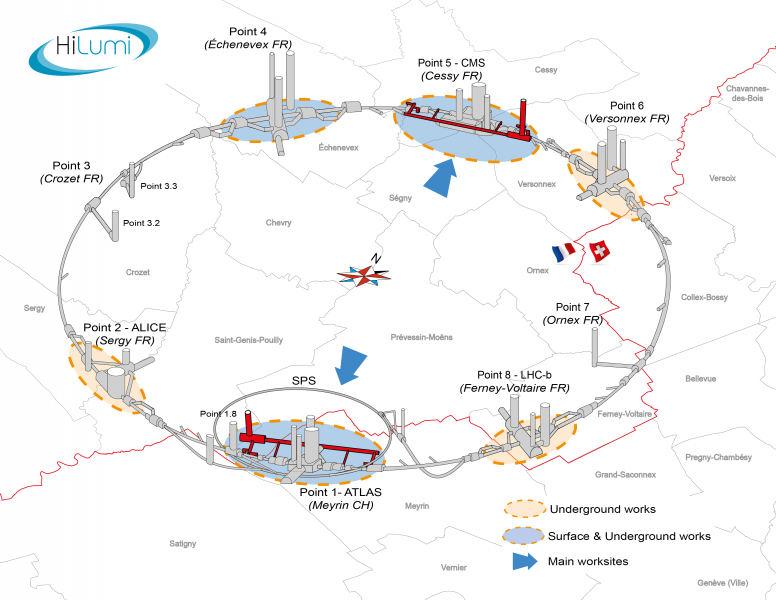
\includegraphics[width=0.75\textwidth]{figures/chapter_ATLAS/LHCOnBorder}
        \caption{
			This figure shows where the CERN is located geographically, across the border between France and Switzerland. \cite{Brüning:782076} 
        }
        \label{fig:CERNAcceleratorComplex}
        \ref{LHCOnBorder}
    \end{center}
\end{figure}

The collider was a planned successor to the Large Electron Positron(LEP)(209 GeV collision) and the Tevatron collider(1TeV) in Fermilab. The community converged on a consensus on a O(10)TeV scale collider on proton collision to probe electro-weak scale Higgs boson along with other BSM physics.

The LHC reuses the same tunnel as the LEP experiment, some major modifications were done to the tunnel for the upgrade: To achieve a higher center-of-mass energy, the angular velocity of the particle colliding will need to be increased. The existing magnet from the LEP experiment was replaced to make way for more powerful cryogenic-based super-conducting magnets to bend higher speed particles. The NbTi superconductors provide up to 8T at about 2Kelvin with liquid helium. In addition, as the LHC uses proton-proton beam rather than electron position in the LEP, an extra beam pipe
is therefore needed as the proton beams could not share the same beam pipe as the position-electron beams in the LEP, the radio frequency system is also modified in the upgrade to the LHC to allow for acceleration of the two separate beams. 

% insert picture to the beam pipe

After the upgrade, the main ring of allows for particle collision to happen in 4 main intersection points. These four points are directly inside the four major experiment of ATLAS, CMS, LHCb and ALICE. ATLAS and CMS are general purpose detectors, the data collected are used for studies including Standard Model measurement, Higgs property measurement as well as exotic and new physics searches. The similar but slightly different detector structure between the two experiment allow for cross check
and validation of physics results. All data in these analyses are taken from the ATLAS experiment. 
Other than ATLAS and CMS, ALICE is optimized to study strong physics in the quark gluon plasma generated from lead-lead collision. LHCb is a forward detector that specializes in b(bottom quark related)-physics measurement. Studies on the bottom quark done in LHCb measures CP violation parameter and could matter-antimatter asymmetry of the universe. 

In addition to the four major experiments, the LHC current host four more experiment. LHCf looks for forward particles that originate from cosmic radiation; FASER are experiments to look for long lived exotic particles with lifetime beyond the ATLAS detector; MoEDAL, which sits in the cavern of LHCb and looks for the magnetic monopole or highly ionizing stable massive particles (SMP); TOTEM shares the CMS interaction point, and measures the total
cross section, diffraction process and elastic scattering processes of particles in the proton collisions. The LHC is the largest machine human has ever built, and it's unparallel in the amount of data generated for fundamental physics research and the front of physics that it covers. 

The LHC is designed to operate at a center-of-mass energy of 14 TeV. Protons that gets collided at the different interaction points goes through many stages before its collision. The section below follows the different parts of the Large Hadron Collider from proton production, to its acceleration to its eventual proton collision in the middle of the ATLAS detector. 

\begin{figure}[!htb]
    \begin{center}
        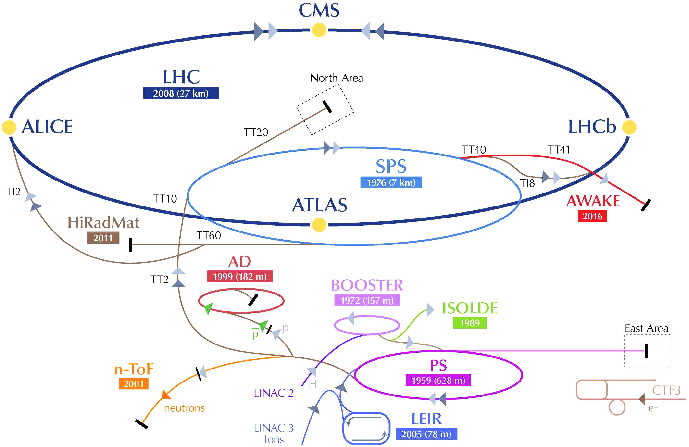
\includegraphics[width=0.75\textwidth]{figures/chapter_ATLAS/LHCAcceleratorComplex}
        \caption{
			This figure shows the accelerator complex of CERN, featuring the experiments and injection chain of the LHC. It also includes experiments outside of the LHC ring like AD and LINR. ~\cite{Marcastel:1621583}.
        }
        \label{fig:CERNAcceleratorComplex}
    \end{center}
\end{figure}

%Image of the LHC Rings


\subsection{Proton Production}
The protons collided in the LHC came from hydrogen in gaseous form. They are stripped out the electron by going through duoplasmatron ion sources, and protons formed are grated to make sure they are of the same direction before being sent off to the injection chain for acceleration. 

\subsection{The Injection Chain}
The preparation of proton after their production to ready for the LHC is called an injection chain process, it mainly consist of a series of pre-acceleration steps through different booster rings. As angular frequency and thus speed and energy of the particle is restricted by both the acclerator ring size as well as magnet size, a dedicated series of smaller rings in ascending order in size are used to accelerate the beam to higher energy level before the LHC ring.

The protons first go through a linear acclerator named LINAC2 to be acclerated to 50 MeV. After the acceleration, they enter a synchrontron ring called the PS Booster, the protons are acllerated to 1.4 GeV. Subsequently, they are injected into the Proton Synchrotron(PS). The PS accelerate the proton further to  26 GeV and injected into the Super Proton Synchrotron(SPS), the proton are then further accelerated to 450 GEV and passed onto the LHC ring in bunches.  

These booster rings are exisitng structures from previous collider experiments. They each specializes in a fixed range of acceleration. 

\begin{figure}[!htb]
    \begin{center}
        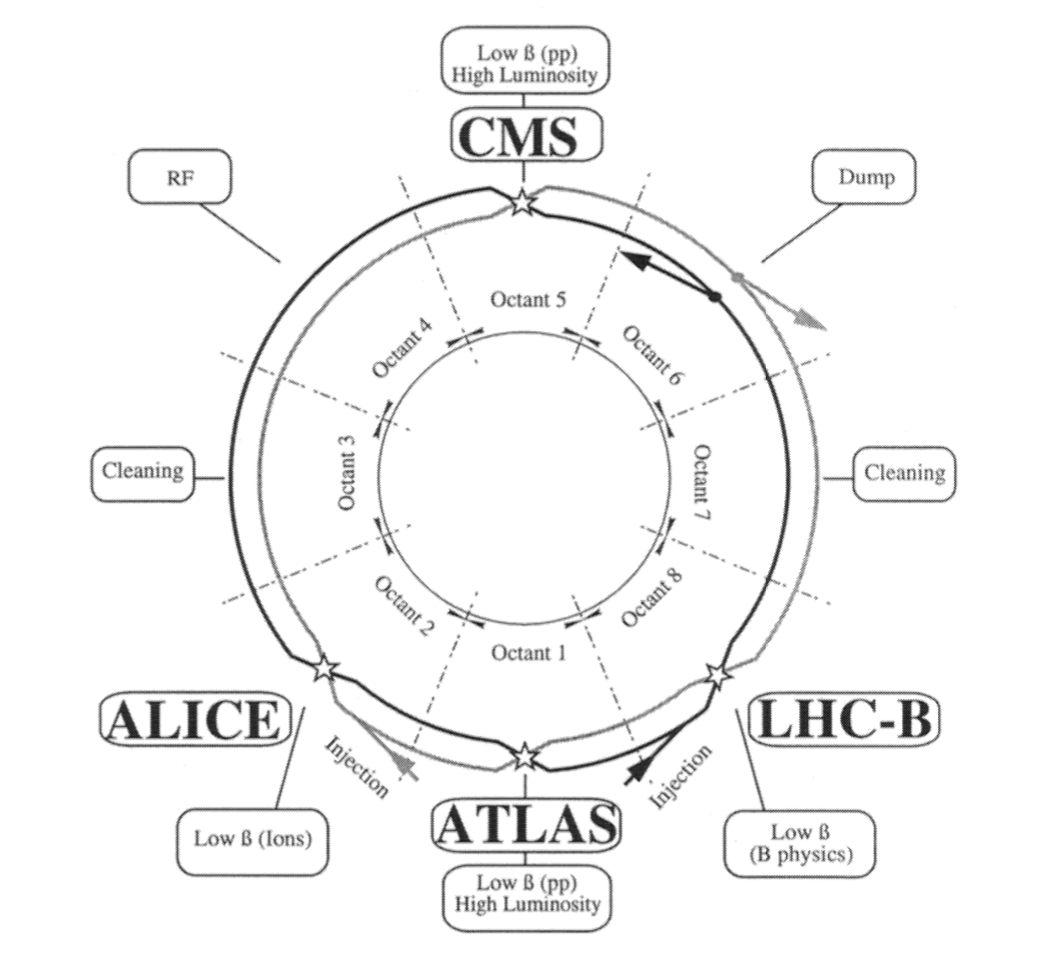
\includegraphics[width=0.75\textwidth]{figures/chapter_ATLAS/LHCRing}
        \caption{
			This figure shows the different parts of the two LHC rings along with its features. ~\cite{Pettersson:291782}.
        }
        \label{fig:perterson}
    \end{center}
\end{figure}

\subsection{The Radio Frequency Cavities}
Located in IP4 of the LHC main ring, the radio frequency(RF) cavity of the LHC performs the acceleration of particles in the ring. The cavity oscillates its electric field at a fixed 400MHz rate, which accelerate the incoming well-timed protons. Protons that arrive in the LHC are accelerated from the 450 GeV injection energy to 6.5 TeV in 10 million loops around the LHC, which takes approximately 20 minutes. Other than accelerating proton, the cavaty the protons'
energy are also modulated by the RF cavity, where slowed proton are accelerated and fast one decelerated. They are modulated into proton "bunches" for collision. 

\subsection{The Beam Dump}
The beam dump of the LHC is located in IP6 og the ring. Designed to abort the beam for when an issue occured. The designed is made to minimize damage done to the entire LHC system. 

\subsection{The Magnets}
The Magent systems in the LHC offers a way to control the proton beam after its injection from the SPS. The magents bend the proton beams for them to stay on the circular cyclotron tunnels as well to focus and align the beam for collision for maximal interaction rate. Due to the high bending power needed, the main ring of the LHC uses NbTi superconducting magnets.  A supporting cryostatics system cools the magents down to 1.9K. The main dipole system is shown to be able to provide a magnetic field of up to 8.4T under this condition. There are a couple of different kinds of magnets along the
LHC, each providing a different function in maintaining the beam for particle collision. The field quality can be summarized by the harmonic multipole analysis: 

\[ B_y+ iB_x  = B_1\sum_n(b_{n} + i a_{n})(Z/R_{r})^{n-1}\]
where B_y is the dipole field in the y direction, $b_{n}$ and $a_n$ is the normal and skwed multipole coefficient, Z is a complex number that describes the coordinates of the magnet, $R_{r}$ is the reference radius. The index of n=1 refers to the dipole file, n=2  refers to the quadrapole field and so on. 


\subsubsection{The Main dipole magnets}
The main magnet are dipole magnets that bends the proton beam to make them stay on track in the circular tunnels. It can also be used to control the separation of the beam as it enter and exist different parts in the main ring. 
The LHC have two beam pipe for each proton beam going in opposite direction from the other. The Magnet has a twin-aparature system that allows it to bend both proton beams together. Figure~\ref{fig:dipole} shows the cross-section of the dipole magnet. 



\subsubsection{The Quadrapole and sextupole magnets}
The Quadrapole magenets are also used in the LHC, to focus and defocus the proton beams for collision, they are also built in a two-in-one system much like that of the main dipole. Figure~\ref{fig:quadrapole} shows a cross section of the quadrapole magnet. 

\subsubsection{The Sextupole and dipole corrector magnet}
In addition, there are corrector magnets that corrects for the field error of the main magets mentioned above. More design details can be found in the conceptual design report of the LHC~\ref{}





\subsubection*{Luminosity}

The instantaneous luminosity is a measure of how much event can be produced under certain detector condition, it's directly related to the event rate of different processes under production.   
The quantity is given as the following:

\[ L = \frac{F \cdot N^{2}_{p} n_{b} f_{\lambda}}{4\pi\epi \Beta^{*}}\]
\[ \rightarrow = \frac{N_{proton in beam 1} \cdot N_{proton in beam 2} \cdot Beam Crossing frequency}{Beam overlap Area}

In the formula above, Np is the number of proton in each beam, n_{b} is the number of bunches per beam, f is the frequency of the beam travelling around the collider, and gamma is the relativistic factor, \Beta^{*} is the beam cross sectinoal size at the injection and \epi is the beam emittance. F is the beam crossing angle if there is a one.

The LHC was made to have a peak luminosity at L=2 \cot 10^{34}cm^{-2}s^{-1}, but in run II, it was made to be at 10^{34}cm^{-2}s^{-1}.

While the instantaneous luminosity is a measure of LHC performance in operation, integrated luminosity, denoted by $\mathcal{L} = \integrate L dt$ is a measure of the amount of data taken over a period of time. 

While an increase in instantaneous luminosity increases the event rate in the experiment, it also increases the pile up, which is multiple occurance of events that happened simutaneously as the target events. Pile-up cleaning will therefore become an increasingly important task as the LHC instantaneous luminosity goes up. This will be further discussed in the object identification section. 
%in time vs out of time pile up. 
%TODO updated operation picture, summary integrated luminosity, of run 2 period and the pile up profiling 

%\subsubection*{Bunch Crossing Scheme}
%The bunch crossing scheme of the LHC is as following, 


\section{The ATLAS Detector}
\label{ATLAS}

The ATLAS detector is a general purpose detector designed for multiple purposes, it is the summation of a series of detector system each produce different tracks to particle. The ATLAS detector has a special emphasis on the muon system as that was a main channel for the Higgs discovery. In the following section, different part of the detector will be discussed in detail. 

\begin{figure}[!htb]
    \begin{center}
        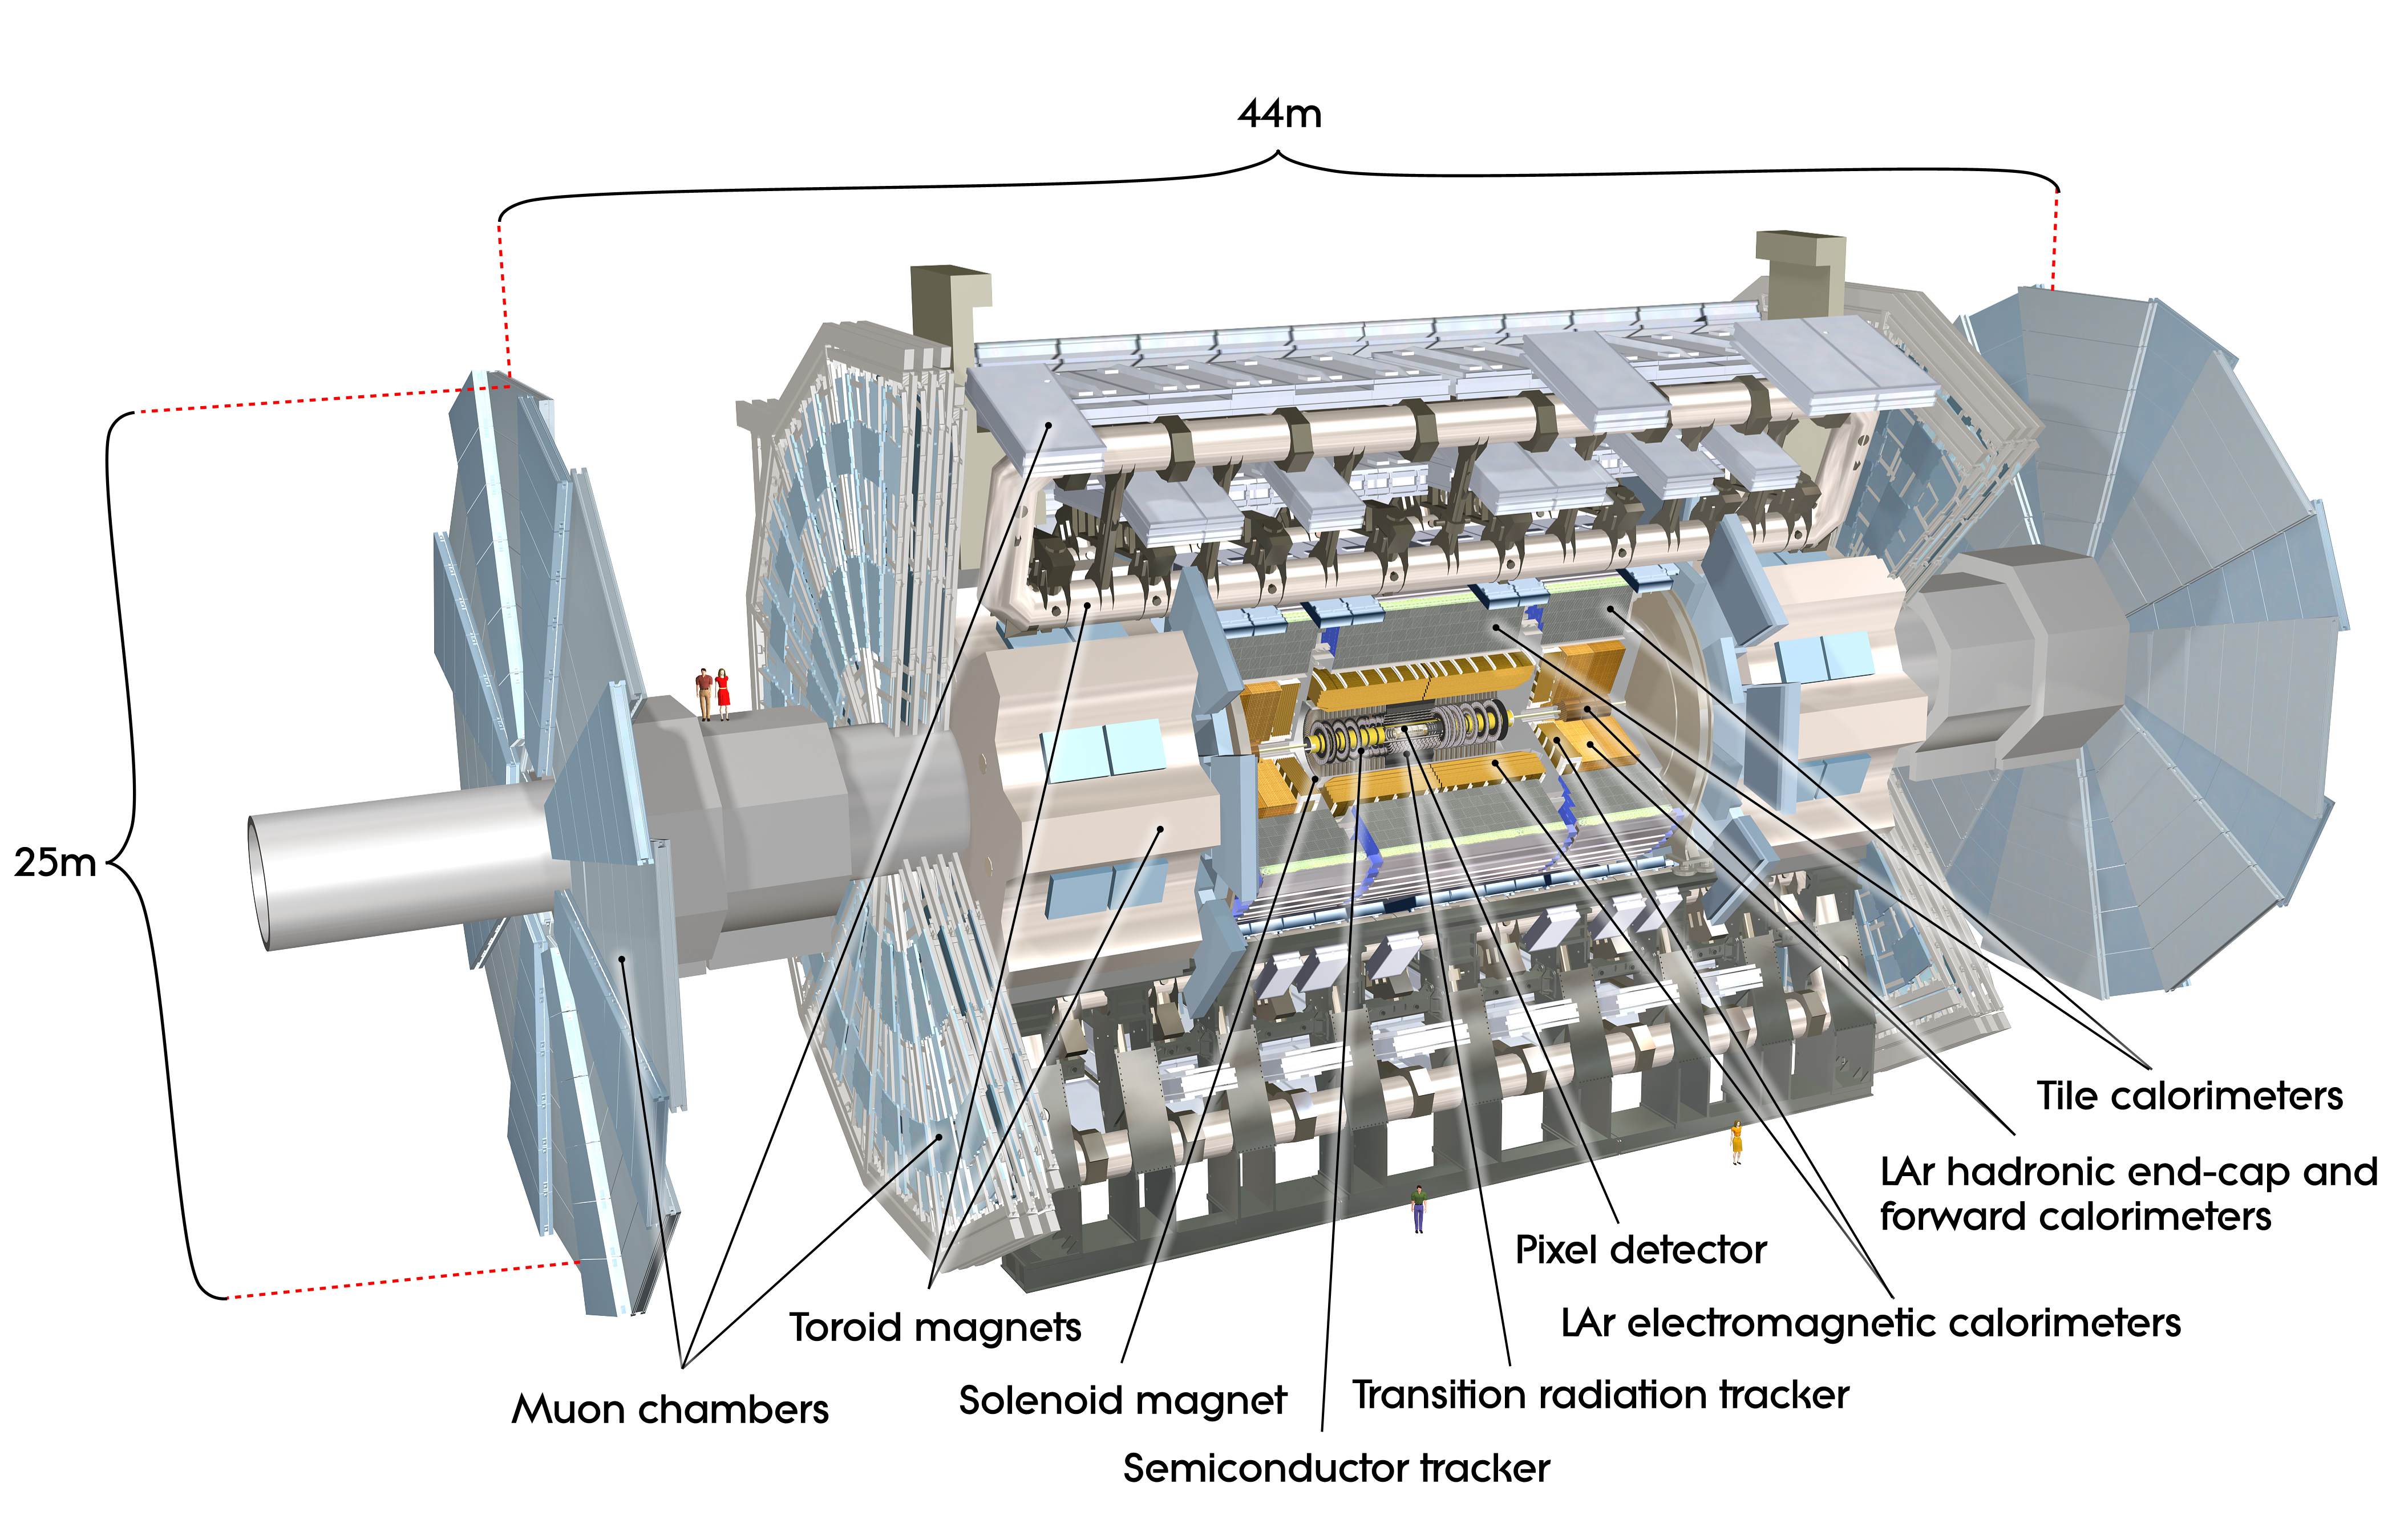
\includegraphics[width=0.75\textwidth]{figures/chapter_ATLAS/ATLASDetector}
        \caption{
			Computer generated image of the ATLAS detector\cite{Pequenao:1095924}. Showing the different parts of the components involved. 
        }
        \label{fig:Coordinates}
        \ref{ATLASCoordinates}
    \end{center}
\end{figure}


\subsection*{The ATLAS coordinate system}

The ATLAS uses a cylindrical coordinate system: Z-\phi-\eta to describe the particles location after interaction.
The z-axis runs along the beam line and starts at the origin (center and middle) of the detector. The x-y plane perpendicular to the z-axis described as the transverse plane is represented in the polar coordinate. The plane is described by two angles: \phi is the 2\pi azimuthal angle on the x-y plane and the 1\pi polar \theta angle with respect to the z axis is given in term of psuedo rapidity, the term is Lorentz invariant and is its conversion to theta is give by: $\eta=ln[tan(\theta/2)]$. The quantity $\deltaR=\sqrt{\delta\eta^{2}+
\delta\phi^{2}} $ is used to describe the angular distance between particles. This quantity is approximately Lorentz invariant. 

\begin{figure}[!htb]
    \begin{center}
        \includegraphics[width=0.75\textwidth]{figures/chapter_ATLAS/ATLASCoordinates}
        \caption{
			This figure displays the coordinate of the ATLAS detector system. \cite{2008} 
        }
        \label{fig:Coordinates}
        \ref{ATLASCoordinates}
    \end{center}
\end{figure}

\begin{figure}[!htb]
    \begin{center}
        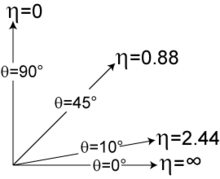
\includegraphics[width=0.75\textwidth]{figures/chapter_ATLAS/pseudorapidity}
        \caption{
			Pseudo-rapidity \eta to angle in degree conversion. \cite{enwiki:1052183914} 
        }
        \label{fig:pseudorapidity}
        \ref{pseudorapidity}
    \end{center}
\end{figure}



\subsection{Inner Detector}
The inner detector(ID) is the innermost part of the ATLAS detector. Its main function is to record charged particle trajectory. The tracks provides valuable information for the reconstruction of the primary vertices of particle interactions. All four parts of the ID enclosed by a superconducting solenoid magnet of 2T aligned along the beam line, charged particles are curved into a helical trajectories along the beamline. This is be used for charge, mass and momentum calculation as well as particle
identification. 

% TODO insert charge to mass trajectory calculation

The inner detector is made up for four different part. From inside out, the Insertable B Layer, the Pixel detector, the Semi-Conductor Tracker(SCT) and the Transition Radiation Tracker(TRT). 
Its resolution is the highest in the innest part of the detector and decreases outward. The following is a detailed description on the four parts on their coverage and detector mechanism. 

Closest to the core of the detector is a very high resolution insertable B layer(IBL) is inserted after Run I to further extend the pixel detector coverage to $|\eta|< 2.9$. This helps with b-hadron identification through better vertex reconstruction. 

Around the IBL is the Pixel detector. It is made of three layers of fine silicon pixels of spatial resolution of 10\mu m in the r-\phi direction 115\mu m in the z direction. It provides a cylindrical coverage that covers up to $|eta|<2.5$. Electron-hole pairs are generated when charged particle passes through the silicon pixel which the signal is then read out through the applied electric field
Surrounding the pixel detector, there is a silicon microstrip detector called the Semi-Conductor tracker (SCT), located in radii between 30-51 cm, which makes up of 4 layers of strip silicon sensor. Each SCT later is made up of two overlapping sets of silicon stips at an angle with one another. The working mecahnism of the detector is similar to that of the pixel detector, but the resolution is slightly reduced to 17 \mum in the r-\phi plane and 580 \mu m along the z axis. 
The outermost part of the ID is called the Trasition Radiation Tracker(TRT), it's made up of gas-filled straws. There are 70 layers in the barrel and 140 layers in each end cap covering up to $|\eta|<2.0$. Each straw tube contains gas that can be ionized by charged particle, the electron formed in the process will then move toward the charged center of the straw to be read out for momentum, trajectory charge calculation. The TRT also helps with particle identification as charged particles also
emit photon and this probability is related to the Lorentz factor. Lower mass electron emits more photons than charged hadrons. Therefore, this can be used to identify electrons over hadrons on top of track reconstruction. 

The TRT has a resolution of 130\mu m in the r-\phi plane. 

\section{Calorimeter}
The main function of the calorimeter is to provide energy measurement of the particles formed after tracking. The ATLAS Calorimeter is split into two parts, sorting by the particle interaction method, The Electromagnetic-Calorimeter(E-Cal) utilizes the electromagnetic interaction and measures energy deposit in the form of electron and photon showers; the Hadronic Calorimeter uses strong hadronic interactions, energy is measured in the form of hadronic shower in quarks and gluons. Both
systems utilizes a dense passive material for the showering and is sampled through a layer of sensitive active element for detection. Below, different components of the ECAL and the HCAL will be described in detail. 

After tracking, the particle will first reach the ECAL, the first layer is the liquid-argon(LAr) electromagnetic(EM) calorimenter. The passive medium for showering is lead. The endcap portion covers $1.375< |\eta| < 3.2$, and the barrel cover up to $|eta|<1.475$. The inner most layer has the greatest granularity of 0.003, the second layer has the resolution of 0.025 and the third layer is the most coarse. 

The hadronic calorimeter(HCAL) measures hadron showering in forms of quarks and gluons, the barrel portion is made of a tile calorimeter, it uses steel as the passive element for showering and scintillating tiles as the readout active element and the 

The forward calorimeter end cap uses LAr for both the ECAL and HCAL, but copper-tungsten is used as the passive layer instead. 

\section{Muon Spectrometers}
The muon spectrometer function to measure both the trajectory muons and perform their trigering. The only type of particles that make it pass the calorimeters and reaches the muon spectrometer are either non-interacting particles, or they are the minimum ionizing particles, muons. A tracking and measurement of muons can effectively distinguish them from the non-interacting particle which could be neutrinos or beyond the standard model physics particles like dark matter. 
The muon spectrometer system of ATLAS is surrounded by the superconducting toroid magnets, the barrel toriod provide up to 0.5 T between $1.6 < |\eta|<2.7$ , the end cap toriods provide up to 1T. The magnet bend the particles along the beamline into the end caps.
For precision tracking, the muon system is made up of the Monitored Drift Tubes(MDTs) in both the barrel and the endcap region, in the forward region there is a Cathode Strip Chamber(CSCs) in region $|\eta|>2.7$
For triggering, it uses the Resistive Plate Chamber(RPC) in the barrel and the Thin Gap Chambers (TGCs) in the end cap for fast readout. 

%Comparison with CMS

\section{Data Acquisition of ATLAS}
%Data acquisition of ATLAS 
During Run II of the ATLAS operation, the LHC performed proton-proton collision at 13 TeV at the instantaneous luminosity of 10^{34}cm^{-2}s^{-1}. An approximate of 33.7 pp interaction per bunch crossing was delivered. 
At this collision rate, not all data could be processed and saved. The process of selecting experimentally interesting events is called triggering. In run 2, triggering is administered and controlled by a central trigger processor which assign different information from detector to different part of the trigger computing system. There are two levels of triggering in ATLAS run2 , the low level hardware based trigger is called L1 triggers, the second level software based high level triggering is called the High-level trigger(HLT). 
The L1 trigger filters through the input at 40 MHz to 100kHz. This is done so by looking at energy deposits at the calorimeters that could be
candidate leptons, jets or photons. Muons are triggered from the hits that formed towers in the MS system. 
Events that passes through the L1 trigger will then be passed onto the HLT. The HLT further filters the 100kHz events received to 1kHz for writing to disk for offline analysis. The HLT is made  up of a level 2 trigger (L2) and an event filter(EF). The L2 trigger is hardware based, it further defines region-of-interest in detector and filter events that do not fit the trigger selection criteria. The event filter is software based on the ATHENA ATLAS software, high-level objects is created from
the online information and an event loop is used to discard events that do not fullfill the trigger criteria.
information. 
Events are saved to trigger chain for later analysis, they are sort into different analysis derivations with basic criteria applied for different types of analyses. 

%Trigger efficiency is determined 


\section{The New Small Wheel Upgrade}

%80 million read-out channels


0. Introduction

    What is the LHC
    What is the ATLAS detector
    The LHC


1. Different parts of the ATLAS detector 
    1. Accelerator 
    2. Inner detector
    3. Outer detector
    4. EM calorimeter
    5. Hadronic Calorimeter

2. Triggering system 
2. Particle signature recognition
